% Figure consists of 4 parts (in this order in the code)
% Surface D (upper left)
% Detail plot highlighted square (lower left)
% Surface S (non-linear transformation of surface D) (upper right)
% Detail plot highlighted square on surface S (lower right)
\documentclass{article}
\usepackage{tikz}
\usepackage{float}
\usepackage{lmodern}
\usepackage{amsmath}
\usetikzlibrary{calc}
\usetikzlibrary{intersections}
\usetikzlibrary{decorations.markings}
\usetikzlibrary{arrows, arrows.meta}
\usetikzlibrary{patterns,patterns.meta}
\usepgfmodule{nonlineartransformations}

\begin{document}

\centering

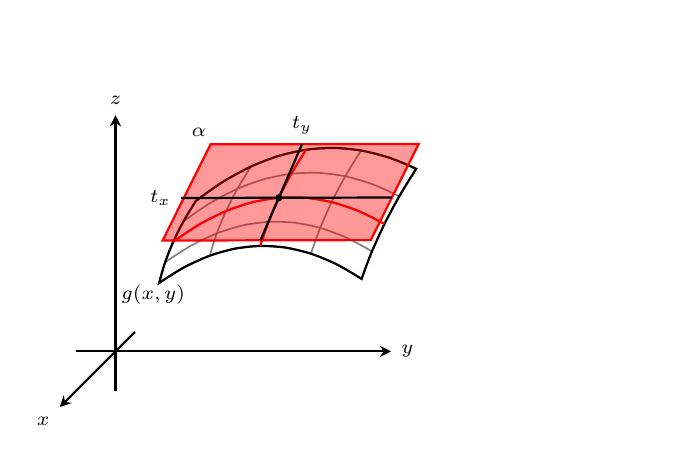
\begin{tikzpicture}[scale=1.0, xshift=1.347cm]  % set scale same as picturescale!
\pgfmathsetmacro{\PictureScale}{1.0}
\pgfmathsetmacro{\CircleSize}{0.03}     % radius of coordinate circles/dots
% conversion from cm to pt and vice versa
\pgfmathsetmacro{\CmToPt}{28.3464566929}
\pgfmathsetmacro{\PtToCm}{0.0352777778}
% define styles used in this picture
\tikzset{every node/.style={font=\scriptsize,text=black},
CircleNodeStyle/.style={draw=black, shape=circle, fill=black, minimum size=\CircleSize*2.5 cm, inner sep=0pt},
arrowstyle/.style={->, >=stealth}}


% second axis
\pgfmathsetmacro{\OvershootAxis}{0.5}
% x and z-axes
\draw[arrowstyle, thick] (-\OvershootAxis,0) -- (3.5,0) node[pos=1, right] {$y$};
\draw[arrowstyle, thick] (0,-\OvershootAxis) -- (0,3.0) node[pos=1, above] {$z$};
% y-axis (angled)
\pgfmathsetmacro{\AngleAxis}{45}
\pgfmathsetmacro{\ZAxisBeginX}{cos(\AngleAxis) * \OvershootAxis * 0.7}
\pgfmathsetmacro{\ZAxisBeginY}{ sin(\AngleAxis) * \OvershootAxis * 0.7}
\pgfmathsetmacro{\ZAxisEndX}{- cos(\AngleAxis)*1.0}
\pgfmathsetmacro{\ZAxisEndY}{ - sin(\AngleAxis) * 1.0}
\draw[arrowstyle, thick] (\ZAxisBeginX, \ZAxisBeginY) -- (\ZAxisEndX, \ZAxisEndY) node[pos=1, below left] {$x$};

% surface D (u and v)
\pgfmathsetmacro{\Startuv}{0.5}
\pgfmathsetmacro{\Endu}{3.5}
\pgfmathsetmacro{\Endv}{2}
\pgfmathsetmacro{\usegments}{4}
\pgfmathsetmacro{\vsegments}{4}
\pgfmathsetmacro{\ustepsize}{(\Endu-\Startuv)/\usegments}
\pgfmathsetmacro{\vstepsize}{(\Endv-\Startuv)/\vsegments}

% u and v index, of highlighted rectangle
\pgfmathsetmacro{\HiglightedIndexU}{2}
\pgfmathsetmacro{\HiglightedIndexV}{2}


% surface S (non-linear transformation of surface D)
% the nonlinear transformation is calibrated on a certain figure
% dimensions of calibrated surface
\pgfmathsetmacro{\XWidthOrig}{7.0}
\pgfmathsetmacro{\YWidthOrig}{7.0}
\pgfmathsetmacro{\StartXOrig}{0.0}
\pgfmathsetmacro{\StartYOrig}{5.0}
% nonlinear parts of the transformation (x^2, x*y...) need to be scaled to calibration size (via "scale") to ensure no deformation (non-linear transformation on figure size 10 won't have same effect as on a figure with size 1)
\pgfmathsetmacro{\Xscale}{(\Endu - \Startuv) / (\XWidthOrig*1.4)}   % original object xdim / calibrated object xdim
\pgfmathsetmacro{\Yscale}{(\Endv - \Startuv) / (\YWidthOrig*1.4)}
\pgfmathsetmacro{\scale}{(\Xscale+\Yscale)/2 * \PictureScale}
\pgfmathsetmacro{\ScopeScale}{0.8}                      % applied zoom-factor (in scope)
\pgfmathsetmacro{\ScaleInScope}{\ScopeScale * \scale}   % resulting scale in scope

% Function: non linear transformation
% nonlinear parts (x^2, x*y, ...) were selected by adding them one by one for desired result
\makeatletter
\def\CustomNonlinearTransformation#1#2#3{%
% #1: x shift
% #2: y shift
% #3: scaling factor
\pgfmathsetmacro{\offsetx}{\pgf@x + #1}
\pgfmathsetmacro{\offsety}{\pgf@y + #2}
\pgfmathsetmacro{\myX}{\offsetx + 0.001*\pgf@y*\pgf@y / #3 + 0.0005*\pgf@x*\pgf@y / #3} %
\pgfmathsetmacro{\myY}{\offsety - 0.002*\pgf@x*\pgf@x / #3 + 0.0008*\pgf@x*\pgf@y / #3} %
\setlength{\pgf@x}{\myX pt}
\setlength{\pgf@y}{\myY pt}
}
\makeatother

% define corners of transformation highlighted square: flip indices for X as image appears to be flipped
\pgfmathsetmacro{\ScaledXOrig}{\StartXOrig * \scale}
\pgfmathsetmacro{\ScaledYOrig}{\StartYOrig * \scale}
\pgfmathsetmacro{\MaxX}{\ScaledXOrig - \ustepsize * (\usegments)}
\pgfmathsetmacro{\MaxY}{\ScaledYOrig + \vstepsize * (\vsegments)}

%% track the position of non-linear transformation with no shift. 
% Resulting position of the tracker is then used to position figure
\def\TrackPosition#1#2#3#4{%
%#1: Tracker x-position
%#2: Tracker y-position
%#3: ScopeScale
%#4: ScaleInScope
\begin{scope}[scale=#3]
    \pgftransformnonlinear{\CustomNonlinearTransformation{0.0}{0.0}{#4}}
    \coordinate (Tracker) at (#1, #2);
\end{scope}
% extract x- and y-dimension
\newdimen\xshiftneg 
\newdimen\yshiftneg
\pgfextractx{\xshiftneg}{\pgfpointanchor{Tracker}{center}} 
\pgfextracty{\yshiftneg}{\pgfpointanchor{Tracker}{center}}
% shift is the inverse of the tracker position
\pgfmathsetmacro{\xshiftOrig}{ -\xshiftneg} 
\pgfmathsetmacro{\yshiftOrig}{ -\yshiftneg}
}

% define x- and y-shift
\TrackPosition{\MaxX}{\MaxY}{\ScopeScale}{\ScaleInScope}
\pgfmathsetmacro{\xshiftTot}{\xshiftOrig + (0.5) * \CmToPt } 
\pgfmathsetmacro{\yshiftTot}{\yshiftOrig + 1.5*\CmToPt}

% define corners of transformation highlighted square: flip indices for X as image appears to be flipped
\pgfmathsetmacro{\HighlightedX}{- \ustepsize * (\usegments - \HiglightedIndexU)}
\pgfmathsetmacro{\HighlightedY}{ \vstepsize * (\HiglightedIndexV)}
% Define begin and end points of lines
\pgfmathsetmacro{\HighlightedMinX}{- \ustepsize * 0}
\pgfmathsetmacro{\HighlightedMaxX}{- \ustepsize * (\usegments)}
\pgfmathsetmacro{\HighlightedMinY}{\vstepsize * 0}
\pgfmathsetmacro{\HighlightedMaxY}{\vstepsize * (\vsegments)}

% need reference points to calculate the derivative close to the highlighted point z0
\pgfmathsetmacro{\epsderiv}{0.5}        % increase (as fraction of stepsize) for derivative calculation
\pgfmathsetmacro{\segmentseps}{1 / \epsderiv} 
\pgfmathsetmacro{\RefX}{\HighlightedX + \ustepsize * \epsderiv}
\pgfmathsetmacro{\RefY}{\HighlightedY + \vstepsize * \epsderiv}

% define offsets for the surface (in pt)
\pgfmathsetmacro{\XOffsetSurface}{15.0}
\pgfmathsetmacro{\YOffsetSurface}{12.0}


% draw surface D and apply non linear transformation -> surface S
\begin{scope}[scale=\ScopeScale, xshift=\ScaledXOrig * \CmToPt, yshift=\ScaledYOrig * \CmToPt, draw=gray]
    \pgftransformnonlinear{\CustomNonlinearTransformation{\xshiftTot *  \PictureScale + \XOffsetSurface}{\yshiftTot * \PictureScale + \YOffsetSurface}{\ScaleInScope}}
    % draw the surface S segments
    \foreach \uindex in {0,...,\usegments}
        \pgfmathsetmacro{\Xcoord}{- \ustepsize * \uindex}
        \pgfmathsetmacro{\YcoordA}{\vstepsize * \vsegments}
        \pgfmathsetmacro{\YcoordB}{0}
        \draw[semithick] (\Xcoord, \YcoordA)--(\Xcoord, \YcoordB);
    \foreach \vindex in {0,...,\vsegments}
        \pgfmathsetmacro{\Ycoord}{\vstepsize * \vindex}
        \pgfmathsetmacro{\XcoordA}{ - \ustepsize * \usegments}
        \pgfmathsetmacro{\XcoordB}{0}
        \draw[semithick] (\XcoordA, \Ycoord)--(\XcoordB, \Ycoord);
    % draw contour of surface D and highlighted square
    \draw[thick, black]  (0, 0) -- ( - \ustepsize * \usegments,  0) -- ( - \ustepsize * \usegments,  \vstepsize * \vsegments) -- (0, \vstepsize * \vsegments) -- cycle;
    \draw[thick, red] (\HighlightedX, \HighlightedMinY) -- (\HighlightedX, \HighlightedMaxY);
    \draw[thick, red] (\HighlightedMinX, \HighlightedY) -- (\HighlightedMaxX, \HighlightedY);
    % Coordinates that are transformed 
    % (nodes don't transform well direclty with nonlinear transformations...)
    \coordinate (FunctionCoord) at (- \ustepsize * \usegments, 0.0);    % coord for S-node
    \coordinate (HighlightedCoord) at (\HighlightedX, \HighlightedY);
    \coordinate (XderivCoord) at (\RefX, \HighlightedY);
    \coordinate (YderivCoord) at (\HighlightedX, \RefY);
\end{scope}     
% place label for the surface S
\node at ($ (FunctionCoord) + (-0.075, -0.15) $) {\scriptsize $g(x,y)$};

% draw plane based on derivatives (as definition tangent plane)
\pgfmathsetmacro{\XMagnifierTop}{\segmentseps * (\usegments - \HiglightedIndexU)}
\coordinate (Xtop) at ($(HighlightedCoord)!\XMagnifierTop!(XderivCoord)$);
\pgfmathsetmacro{\YMagnifierTop}{\segmentseps * (\vsegments - \HiglightedIndexV)}
\coordinate (Ytop) at ($(HighlightedCoord)!\YMagnifierTop!(YderivCoord)$);
% helper coordinates for calculation of plane's corners
\coordinate (Xside) at ($(Xtop) - (HighlightedCoord)$);
\coordinate (Yside) at ($(Ytop) - (HighlightedCoord)$);
% manual adjustments for plane
\pgfmathsetmacro{\CosAngle}{cos(\AngleAxis) }
\pgfmathsetmacro{\SinAngle}{sin(\AngleAxis) }
\coordinate (YsideTop) at ($(Yside) + 0.1*(\CosAngle, \SinAngle)$);
\coordinate (YsideBottom) at ($(Yside) - 0.1*(\CosAngle, \SinAngle)$);
\coordinate (XsideTop) at ($(Xside) + 0.06*(1, 0)$);
\coordinate (XsideBottom) at ($(Xside) - 0.10*(1, 0)$);
% Define coordinates for tangents
\coordinate (UpperMid) at ($(HighlightedCoord) + (YsideTop)$);
\coordinate (MidRight) at ($(HighlightedCoord) + (XsideTop)$);
\coordinate (LowerMid) at ($(HighlightedCoord) - (YsideBottom)$);
\coordinate (MidLeft) at ($(HighlightedCoord) - (XsideBottom)$);

% define plane corners
\coordinate (UpperRight) at ($ (UpperMid) + (XsideTop) $);
\coordinate (LowerRight) at ($ (MidRight) - (YsideBottom) $);
\coordinate (LowerLeft) at ($ (LowerMid) - (XsideBottom) $);
\coordinate (UpperLeft) at ($ (MidLeft) + (YsideTop) $);
% draw the tangent plane
\draw[thick, red, postaction={fill=red, opacity=.4}] (LowerLeft) -- (UpperLeft) -- (UpperRight) -- (LowerRight) -- cycle;
% define intersection for tangents
% for y tangent
\path[name path=UpperSide] (UpperLeft) -- (UpperRight); 
\path[name path=YTangentPath] (LowerMid) -- ($(LowerMid)!5!(HighlightedCoord)$); 
\path[name intersections={of=UpperSide and YTangentPath, by=YTangentIntersect}];
% for x tangent
\path[name path=RightSide] (UpperRight) -- (LowerRight); 
\path[name path=XTangentPath] (MidLeft) -- ($(MidLeft)!5!(HighlightedCoord)$); 
\path[name intersections={of=RightSide and XTangentPath, by=XTangentIntersect}];
% draw the tangent lines
\draw[thick, black, postaction={decorate}, decoration={
    markings,
    mark=at position 1.0 with {\node[above] {$t_y$};}}] (LowerMid) -- (YTangentIntersect);
\draw[thick, black, postaction={decorate}, decoration={
    markings,
    mark=at position 1.0 with {\node[left] {$t_x$};}}] (XTangentIntersect) -- (MidLeft);

% Symbol of tangent plane
\node at ($ (UpperLeft) + (-0.15, 0.15) $) {\scriptsize $\alpha$};

% Position of the point
\node [CircleNodeStyle] at (HighlightedCoord) {};


\end{tikzpicture}

\end{document}